If the stress on an object is larger than a limit decided by the material properties, the object will not only deform, it will also break. If a fracture is to take place it has to be determined where to break the structure. The method used to determine how the elements break is based on a method by O'Brien and Hodgins \cite{fracture} .

This method calculates a stress tensor $\sigma$ for each element. The stress tensor is calculated in equation \ref{stresser}.
 
 \begin{equation}\label{stresser}
 \sigma = EB_{e}\hat{u}
 \end{equation}
 
 A random node in the element is selected a plane is chosen, and the largest eigenvalue of the stress tensor is used to create a plane through that node. The normal of the plane is set to be the eigenvector corresponding to the largest eigenvalue. All elements that share that node are then found, and they are set to belong to the side of the plane where their center of mass is located, as shown in figure \ref{fig:fracture}. The fracture is then created by inserting new nodes and updating the data structure.

\begin{figure}[htbp]
\label{fig:fracture}
\begin{center}
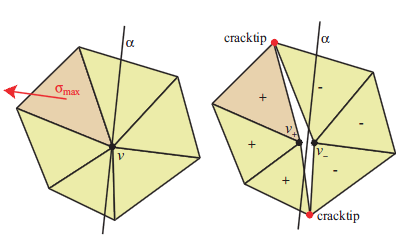
\includegraphics[scale = 0.6]{figures/fracture.png}
\caption{Fracture of nodes}
\end{center}
\end{figure} 